\PassOptionsToPackage{unicode=true}{hyperref} % options for packages loaded elsewhere
\PassOptionsToPackage{hyphens}{url}
%
\documentclass[]{book}
\usepackage{lmodern}
\usepackage{amssymb,amsmath}
\usepackage{ifxetex,ifluatex}
\usepackage{fixltx2e} % provides \textsubscript
\ifnum 0\ifxetex 1\fi\ifluatex 1\fi=0 % if pdftex
  \usepackage[T1]{fontenc}
  \usepackage[utf8]{inputenc}
  \usepackage{textcomp} % provides euro and other symbols
\else % if luatex or xelatex
  \usepackage{unicode-math}
  \defaultfontfeatures{Ligatures=TeX,Scale=MatchLowercase}
\fi
% use upquote if available, for straight quotes in verbatim environments
\IfFileExists{upquote.sty}{\usepackage{upquote}}{}
% use microtype if available
\IfFileExists{microtype.sty}{%
\usepackage[]{microtype}
\UseMicrotypeSet[protrusion]{basicmath} % disable protrusion for tt fonts
}{}
\IfFileExists{parskip.sty}{%
\usepackage{parskip}
}{% else
\setlength{\parindent}{0pt}
\setlength{\parskip}{6pt plus 2pt minus 1pt}
}
\usepackage{hyperref}
\hypersetup{
            pdftitle={FAS OnDemand Quick-Start Guide},
            pdfborder={0 0 0},
            breaklinks=true}
\urlstyle{same}  % don't use monospace font for urls
\usepackage[margin=1.5in]{geometry}
\usepackage{longtable,booktabs}
% Fix footnotes in tables (requires footnote package)
\IfFileExists{footnote.sty}{\usepackage{footnote}\makesavenoteenv{longtable}}{}
\usepackage{graphicx,grffile}
\makeatletter
\def\maxwidth{\ifdim\Gin@nat@width>\linewidth\linewidth\else\Gin@nat@width\fi}
\def\maxheight{\ifdim\Gin@nat@height>\textheight\textheight\else\Gin@nat@height\fi}
\makeatother
% Scale images if necessary, so that they will not overflow the page
% margins by default, and it is still possible to overwrite the defaults
% using explicit options in \includegraphics[width, height, ...]{}
\setkeys{Gin}{width=\maxwidth,height=\maxheight,keepaspectratio}
\setlength{\emergencystretch}{3em}  % prevent overfull lines
\providecommand{\tightlist}{%
  \setlength{\itemsep}{0pt}\setlength{\parskip}{0pt}}
\setcounter{secnumdepth}{5}
% Redefines (sub)paragraphs to behave more like sections
\ifx\paragraph\undefined\else
\let\oldparagraph\paragraph
\renewcommand{\paragraph}[1]{\oldparagraph{#1}\mbox{}}
\fi
\ifx\subparagraph\undefined\else
\let\oldsubparagraph\subparagraph
\renewcommand{\subparagraph}[1]{\oldsubparagraph{#1}\mbox{}}
\fi

% set default figure placement to htbp
\makeatletter
\def\fps@figure{htbp}
\makeatother

\usepackage{booktabs}

\usepackage{epsfig}
\usepackage{epstopdf}
\usepackage{rotate}
\usepackage{graphicx}
\usepackage{hyperref}
\usepackage{alphalph}
\usepackage{caption}
\usepackage[hang,flushmargin]{footmisc}
\usepackage{framed}
\usepackage{xcolor}
\usepackage{verbatim} 

\usepackage{bm}
\setcounter{MaxMatrixCols}{20}
\newcommand{\Var}{\mathrm{Var}}
\newcommand{\SD}{\mathrm{SD}}
\newcommand{\Cov}{\mathrm{Cov}}
\newcommand{\fx}{f({\bf x})}
\newcommand\R{{\textsf R~}}
\newcommand\Rst{\textsf{RStudio}}

% spacing between environments
\usepackage{amsthm}
\makeatletter
\def\thm@space@setup{%
  \thm@preskip=15pt plus 2pt minus 4pt
  \thm@postskip=\thm@preskip
}
\makeatother


% Title format
\usepackage{titling}
\pretitle{\Huge\sffamily}
\posttitle{\par\vskip 0.5em}
\predate{\LARGE\sffamily}
\postdate{\par}

\urlstyle{tt}
\usepackage[]{natbib}
\bibliographystyle{apalike}

\title{FAS OnDemand Quick-Start Guide}
\author{}
\date{\vspace{-2.5em}January 2021}

\begin{document}
\maketitle

{
\setcounter{tocdepth}{1}
\tableofcontents
}
\hypertarget{what-is-fas-ondemand}{%
\chapter*{What is FAS OnDemand?}\label{what-is-fas-ondemand}}
\addcontentsline{toc}{chapter}{What is FAS OnDemand?}

\href{https://atg.fas.harvard.edu/ondemand}{FAS OnDemand} gives Harvard students access to Jupyter Notebooks and RStudio, and can be launched directly from \href{https://canvas.harvard.edu/}{Canvas}. It is hosted by Harvard's FAS Research Computing group (FAS RC) and collaboratively supported by both FAS RC and FAS Academic Technology.

\hypertarget{why-are-we-using-fas-ondemand-for-datafest}{%
\section*{Why are we using FAS OnDemand for DataFest?}\label{why-are-we-using-fas-ondemand-for-datafest}}
\addcontentsline{toc}{section}{Why are we using FAS OnDemand for DataFest?}

It can sometimes be challenging in large courses to get every student's personal computer set-up with the necessary software. For this DataFest bootcamp, you will need an up to date R or Python environment with a suite of non-default packages/modules installed. FAS OnDemand provides you access to an environment that has been curated specifically for DataFest2021, so you can focus on learning skills, rather than debugging your software installation. In addition, you can access FAS OnDemand directly from within the DataFest2021 course on Canvas.

When using the FAS OnDemand environment, you will have access to resources that include:

\begin{itemize}
\tightlist
\item
  8 cores
\item
  16Gb RAM
\item
  20Gb storage
\item
  10Tb scratch storage (shared between all users on the course)
\end{itemize}

Of course, if you prefer to use your own local R or Python environment on your personal computer that is perfectly fine, but we will not be able to provide assistance to you if you encounter problems setting that up correctly.

The FAS OnDemand DataFest2021 Jupyter Notebooks installation comes with a \texttt{Python\ 3} jupyter kernel, common data science packages such as \texttt{numpy}, \texttt{scipy}, \texttt{seaborn}, \texttt{pandas}, \texttt{bokeh}, and \texttt{matplotlib}, as well as many specialized modules we'll use during DataFest.

The FAS OnDemand DataFest2021 RStudio installation is available for \texttt{R\ 4.0.3} and comes preinstalled with common packages such as \texttt{devtools}, \texttt{learnr}, and the complete \texttt{tidyverse} collection of R packages, as well as many specialized packages we'll use during DataFest.

\hypertarget{launch-rstudio-jupyter}{%
\chapter*{Launch RStudio / Jupyter}\label{launch-rstudio-jupyter}}
\addcontentsline{toc}{chapter}{Launch RStudio / Jupyter}

To be able to use the FAS OnDemand computing environment for your DataFest project you will need to walk-through a handful of steps. Once completed, you will be running an RStudio or Jupyter session with all necessary packages pre-installed. The FAS OnDemand computing environment is accessed from \emph{within} Canvas --- look for the \texttt{FAS\ OnDemand} button on the left-side navigation panel. Here are the steps to launch your session:

\begin{enumerate}
\def\labelenumi{\arabic{enumi}.}
\tightlist
\item
  Click \texttt{FAS\ OnDemand} in the left-side navigation panel within Canvas.
\end{enumerate}

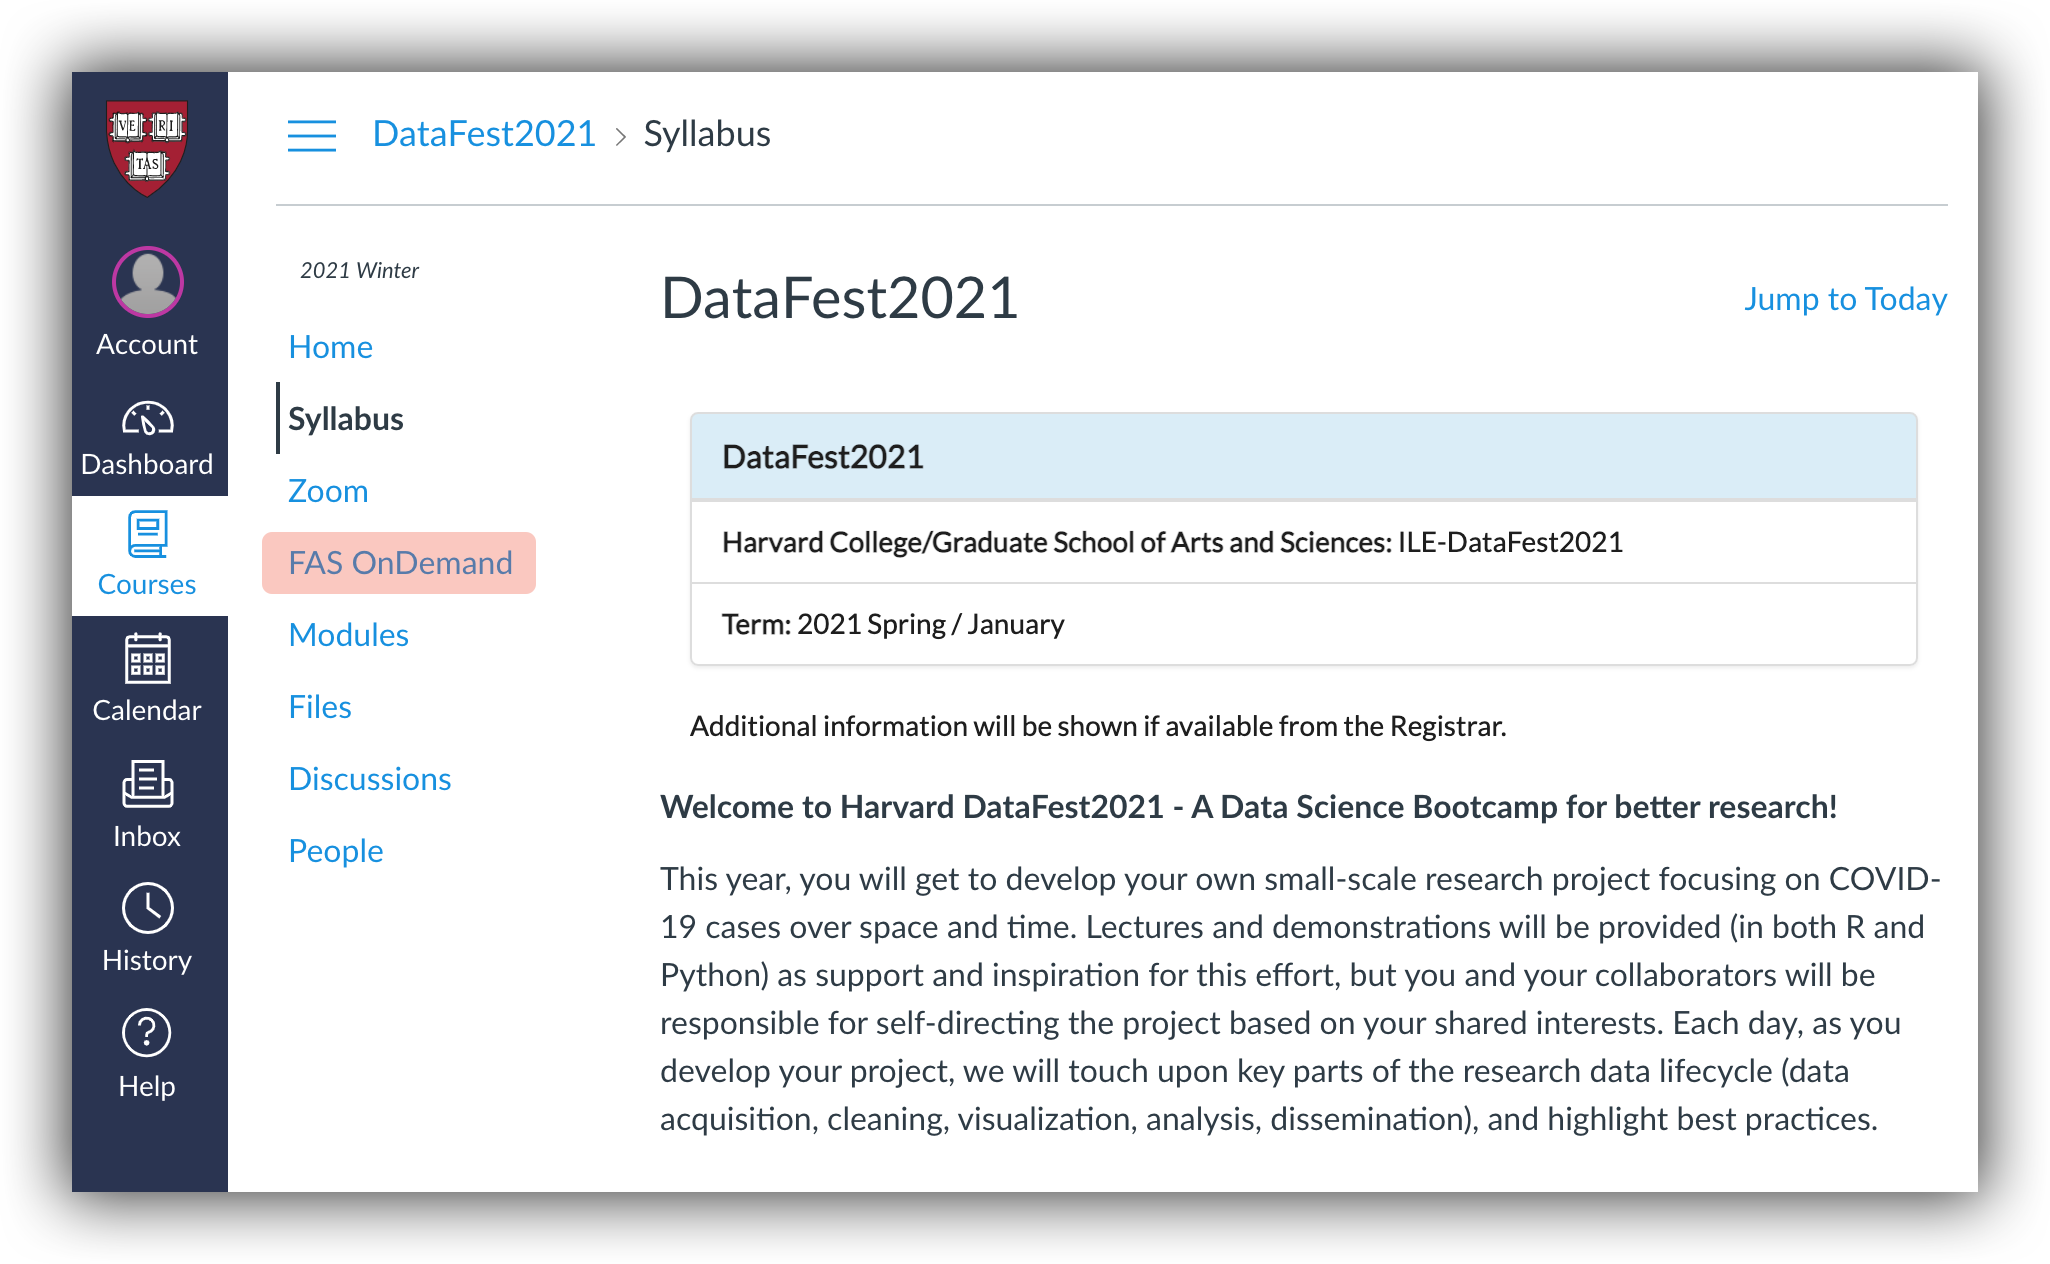
\includegraphics{images/1_canvas.png}

\hypertarget{rstudio}{%
\section{RStudio}\label{rstudio}}

\begin{enumerate}
\def\labelenumi{\arabic{enumi}.}
\setcounter{enumi}{1}
\tightlist
\item
  On the Dashboard launcher page, on the left-side panel, click on \texttt{Rstudio\ Server\ -\ DataFest2021}.
\item
  On the main panel, click the blue \texttt{Launch} button.
\end{enumerate}

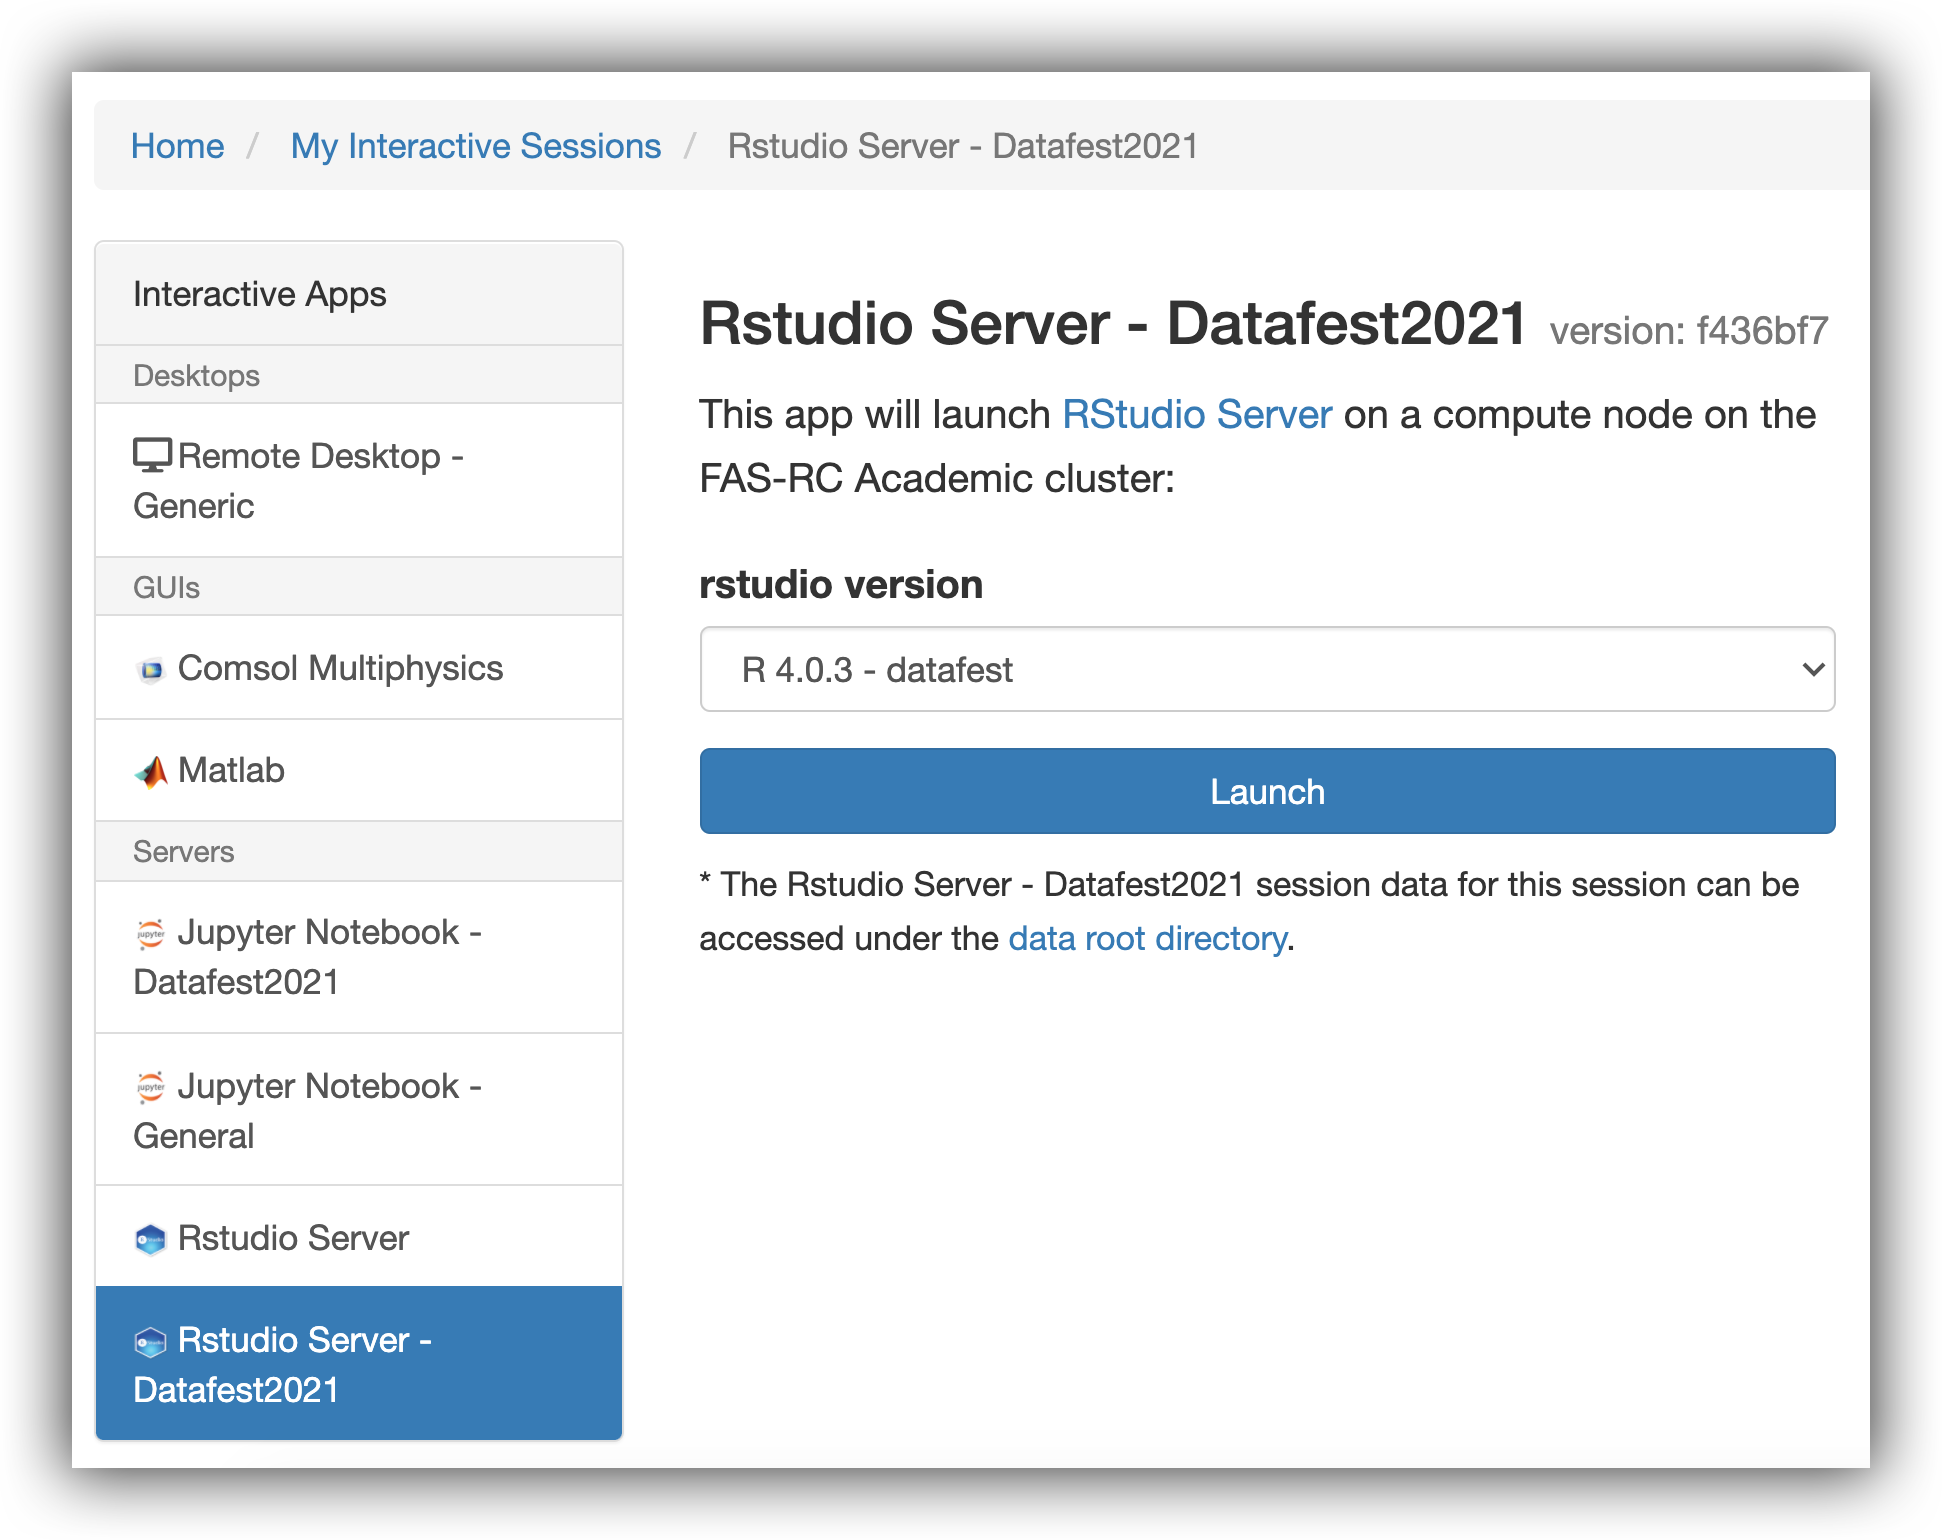
\includegraphics{images/2_launch_rstudio.png}

\begin{enumerate}
\def\labelenumi{\arabic{enumi}.}
\setcounter{enumi}{3}
\tightlist
\item
  On the Sessions page, click on the blue \texttt{Connect\ to\ RStudio\ Server} button.
\end{enumerate}

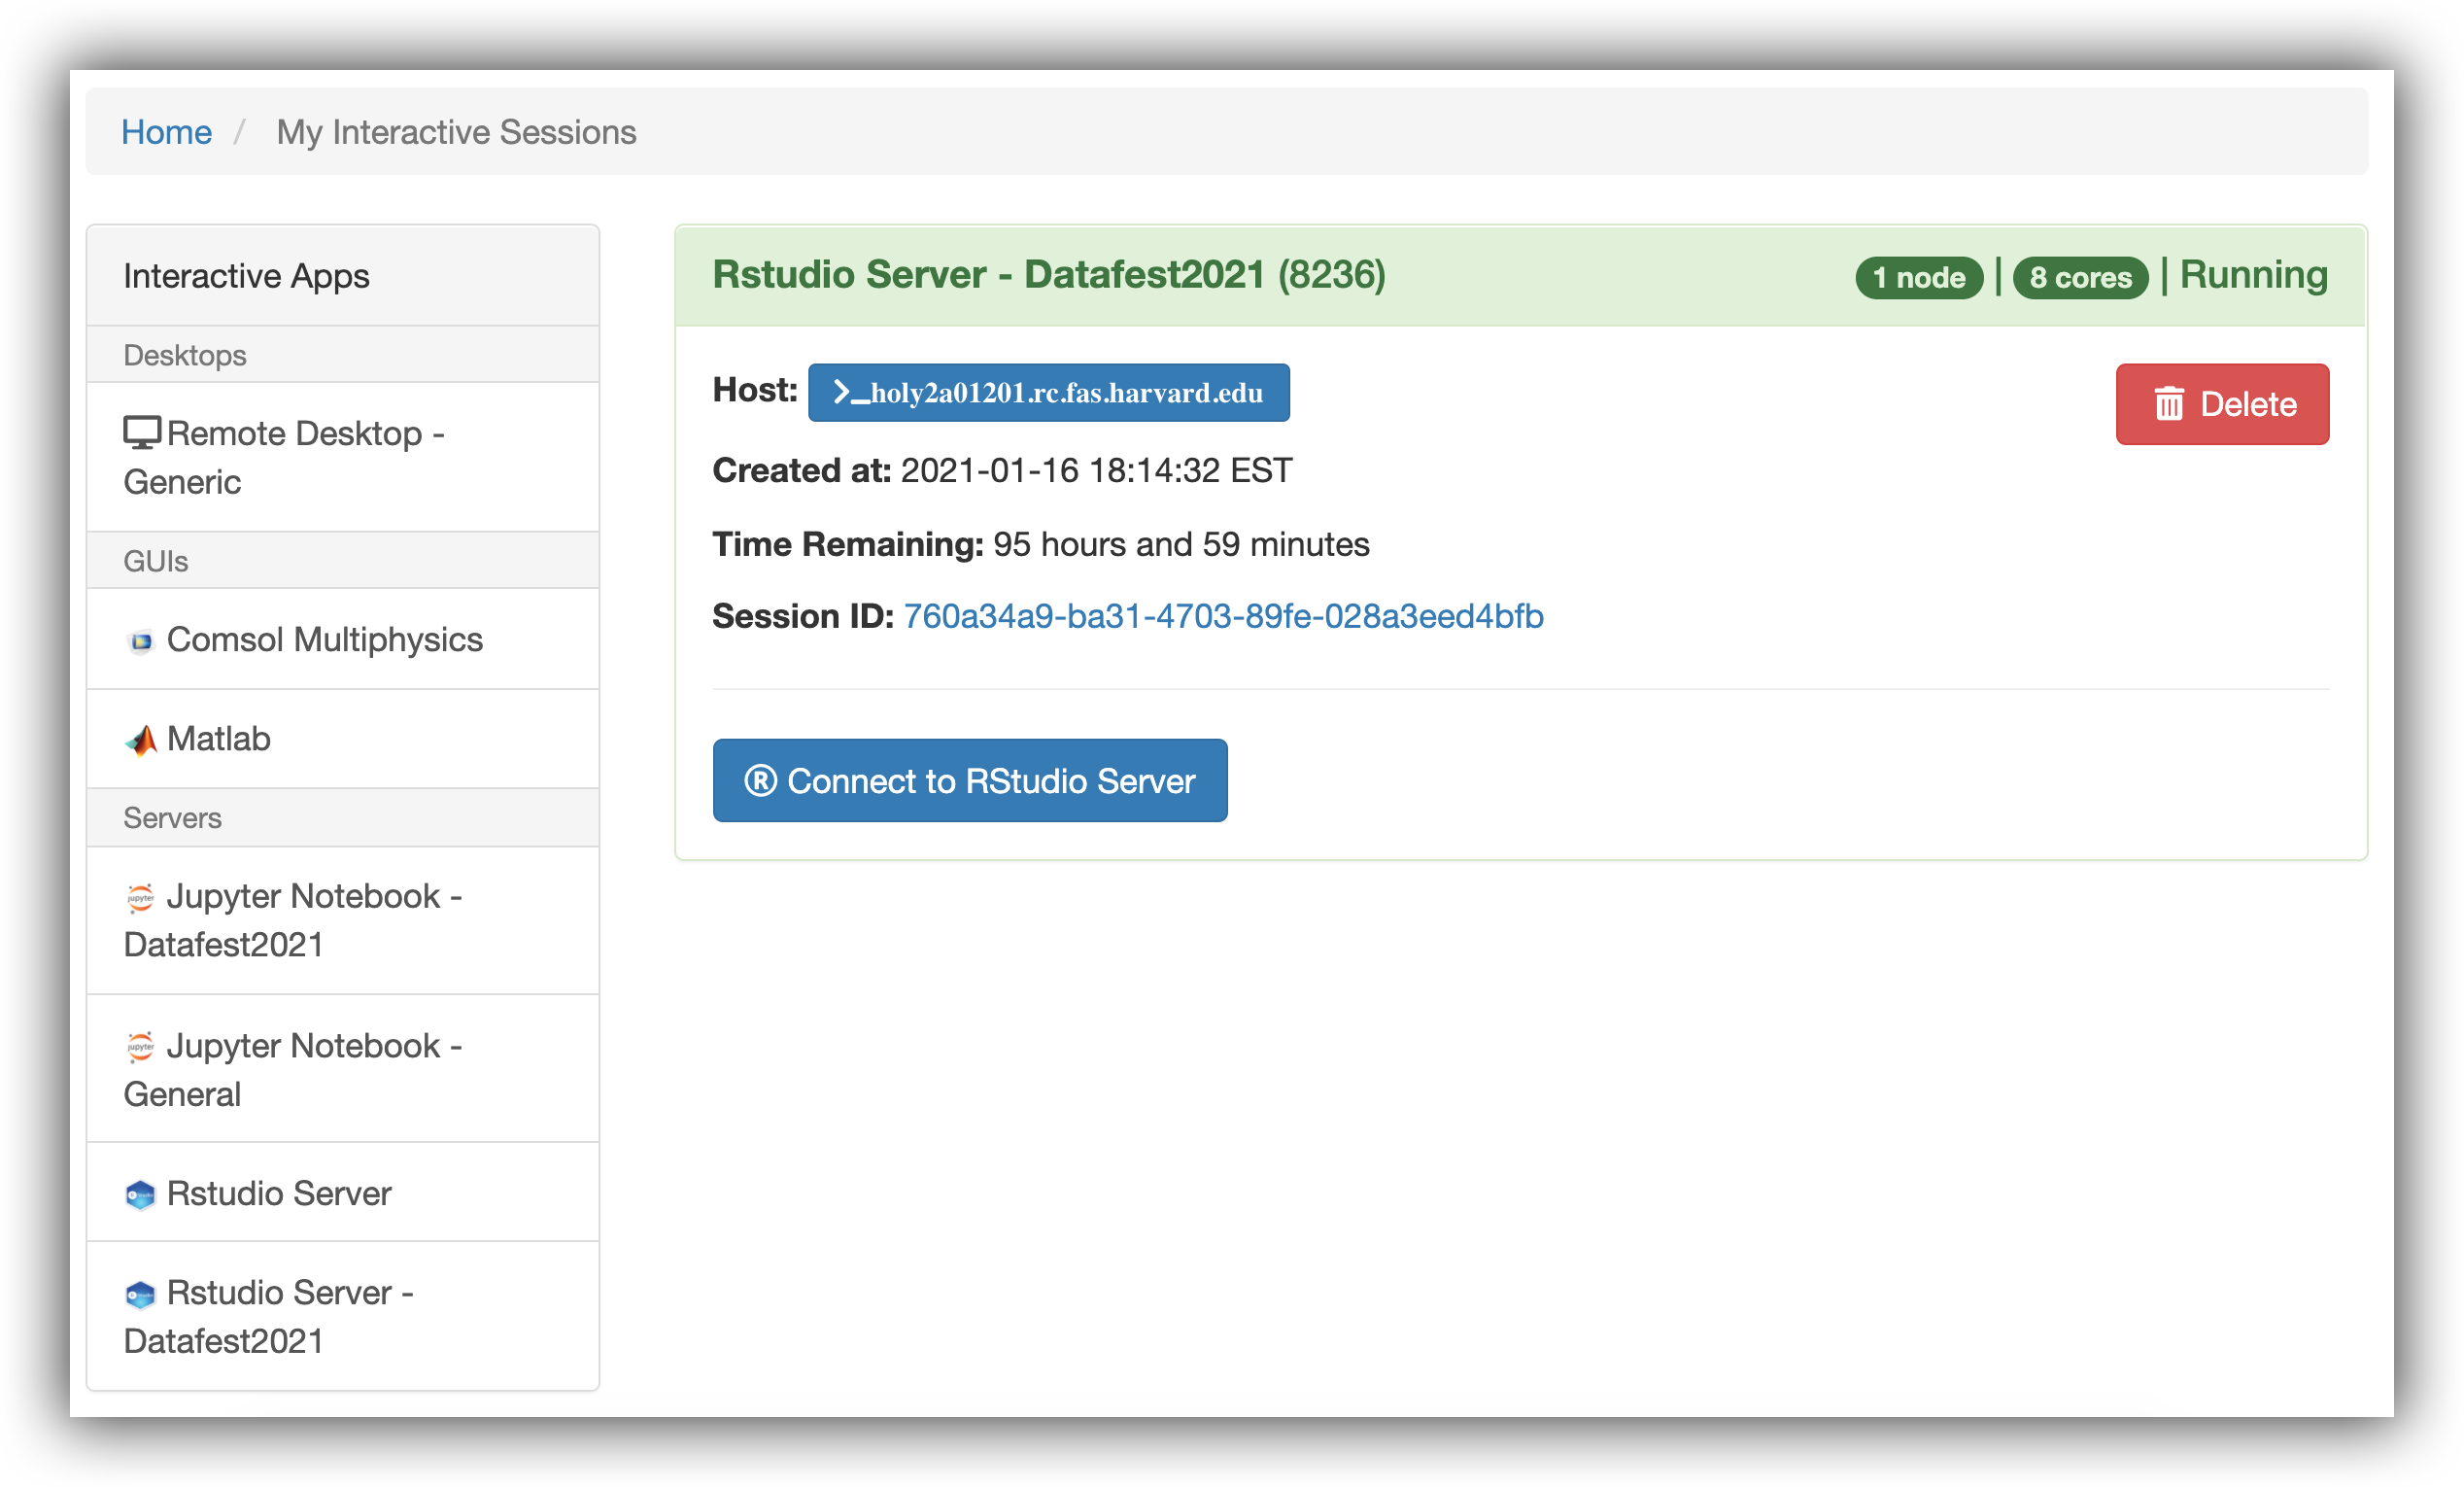
\includegraphics{images/4_connect_rstudio.png}

\begin{enumerate}
\def\labelenumi{\arabic{enumi}.}
\setcounter{enumi}{4}
\tightlist
\item
  You should now have access to RStudio. You can create a new R/Rmarkdown file as usual, or open an existing file.
\end{enumerate}

\hypertarget{jupyter}{%
\section{Jupyter}\label{jupyter}}

\begin{enumerate}
\def\labelenumi{\arabic{enumi}.}
\setcounter{enumi}{1}
\tightlist
\item
  On the Dashboard launcher page, on the left-side panel, click on \texttt{Jupyter\ Notebook\ -\ DataFest2021}.
\item
  On the main panel, click the blue \texttt{Launch} button.
\end{enumerate}

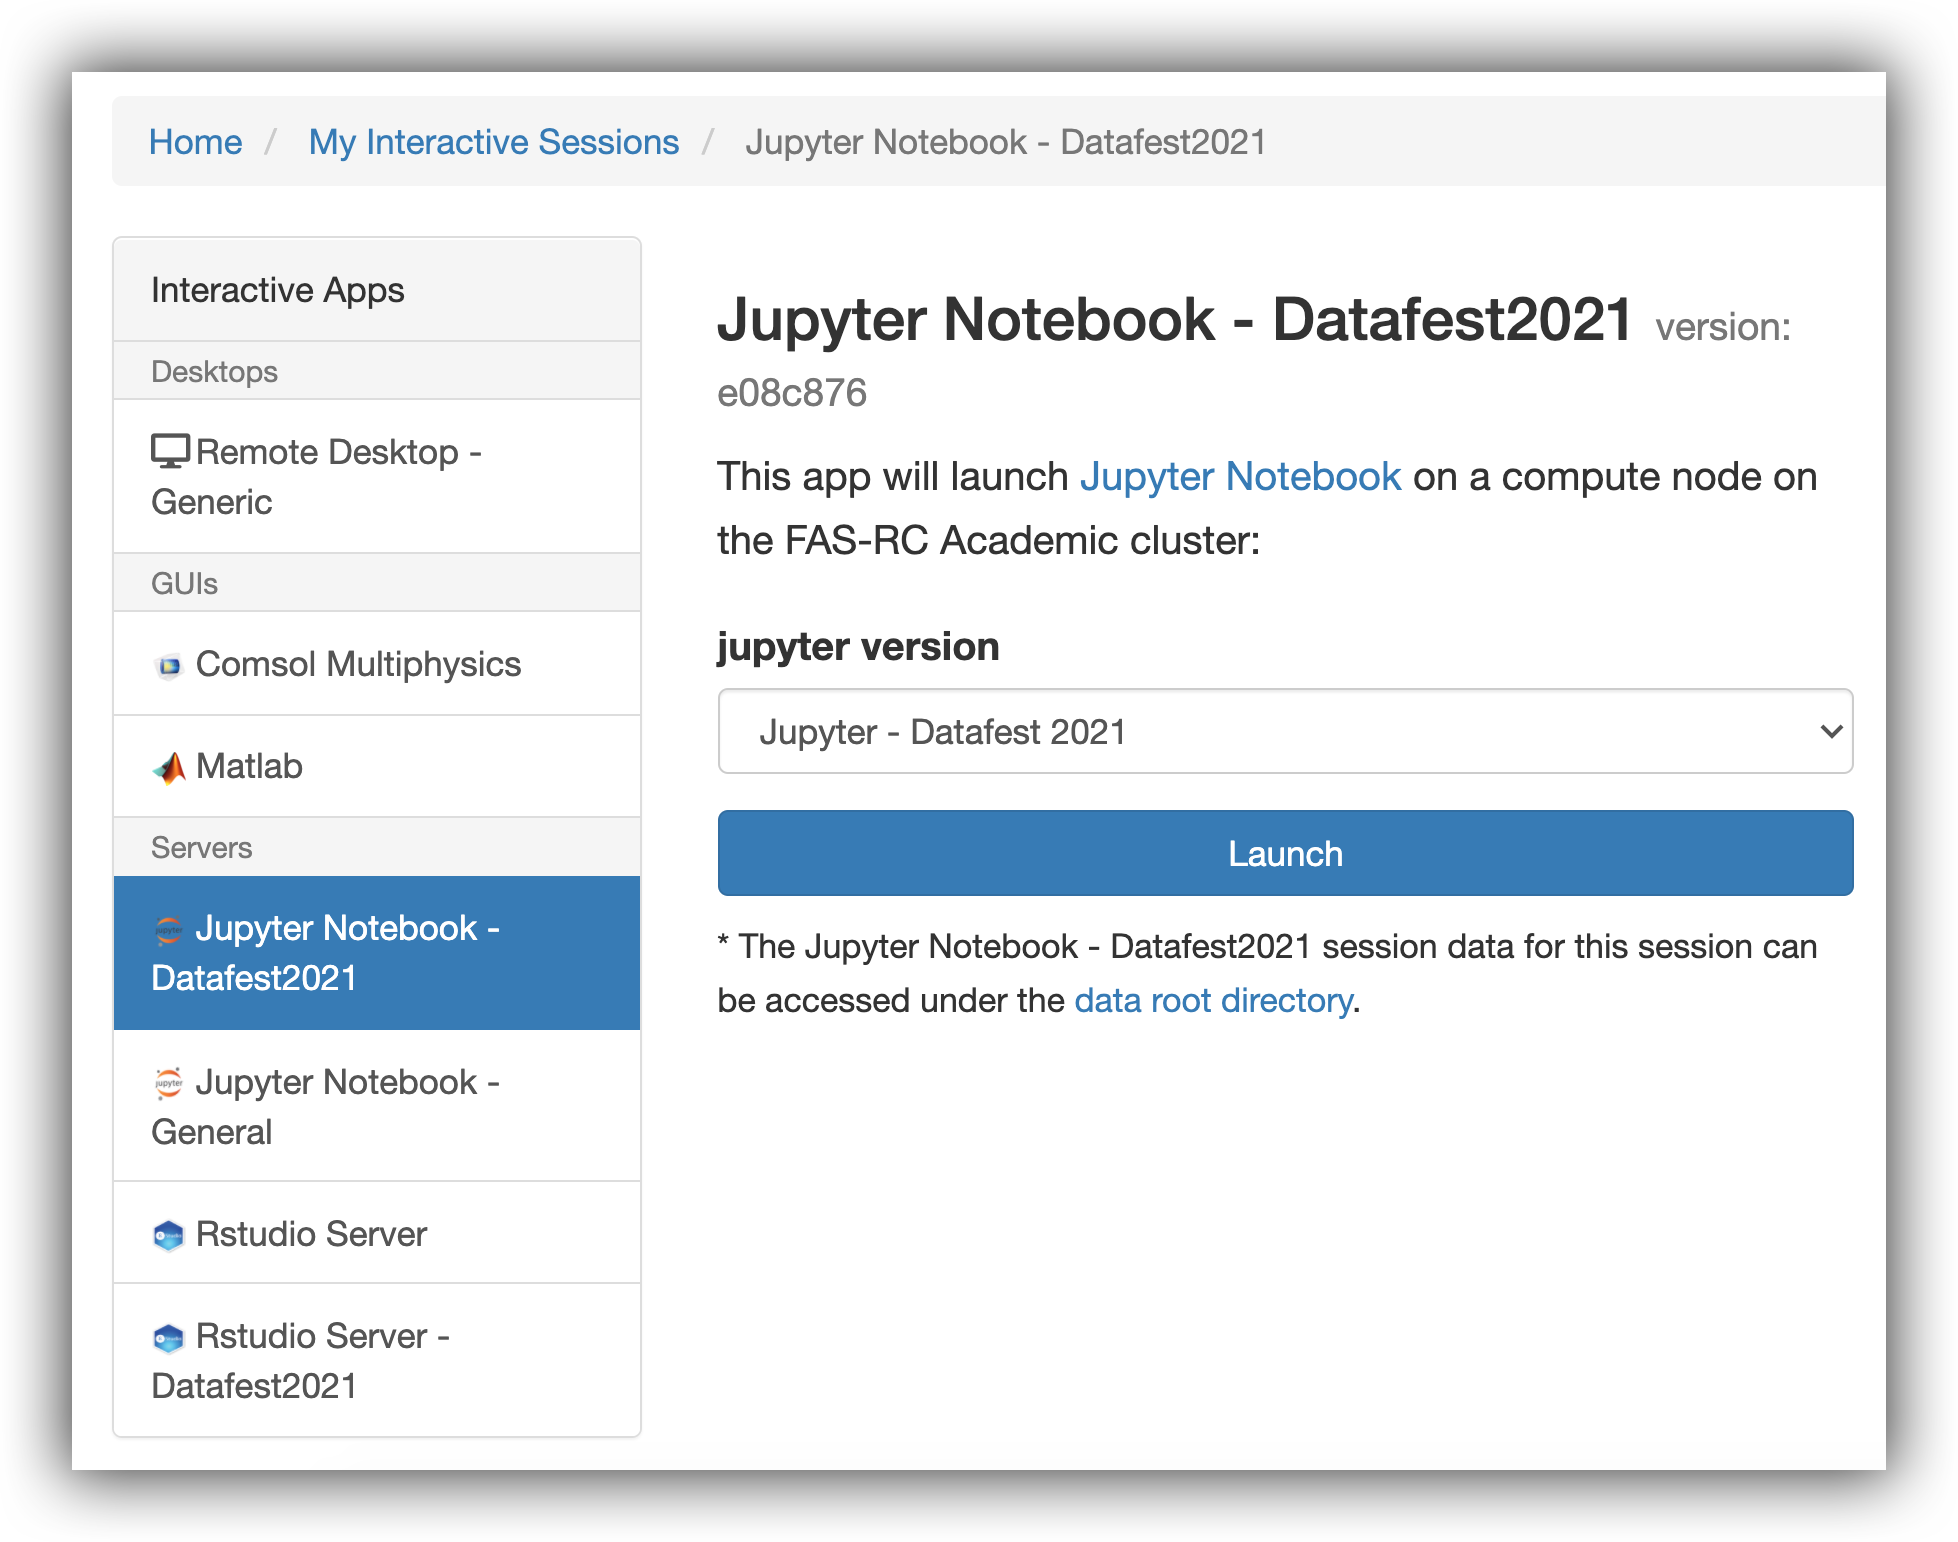
\includegraphics{images/3_launch_jupyter.png}

\begin{enumerate}
\def\labelenumi{\arabic{enumi}.}
\setcounter{enumi}{3}
\tightlist
\item
  On the Sessions page, click on the blue \texttt{Connect\ to\ Jupyter} button.
\end{enumerate}

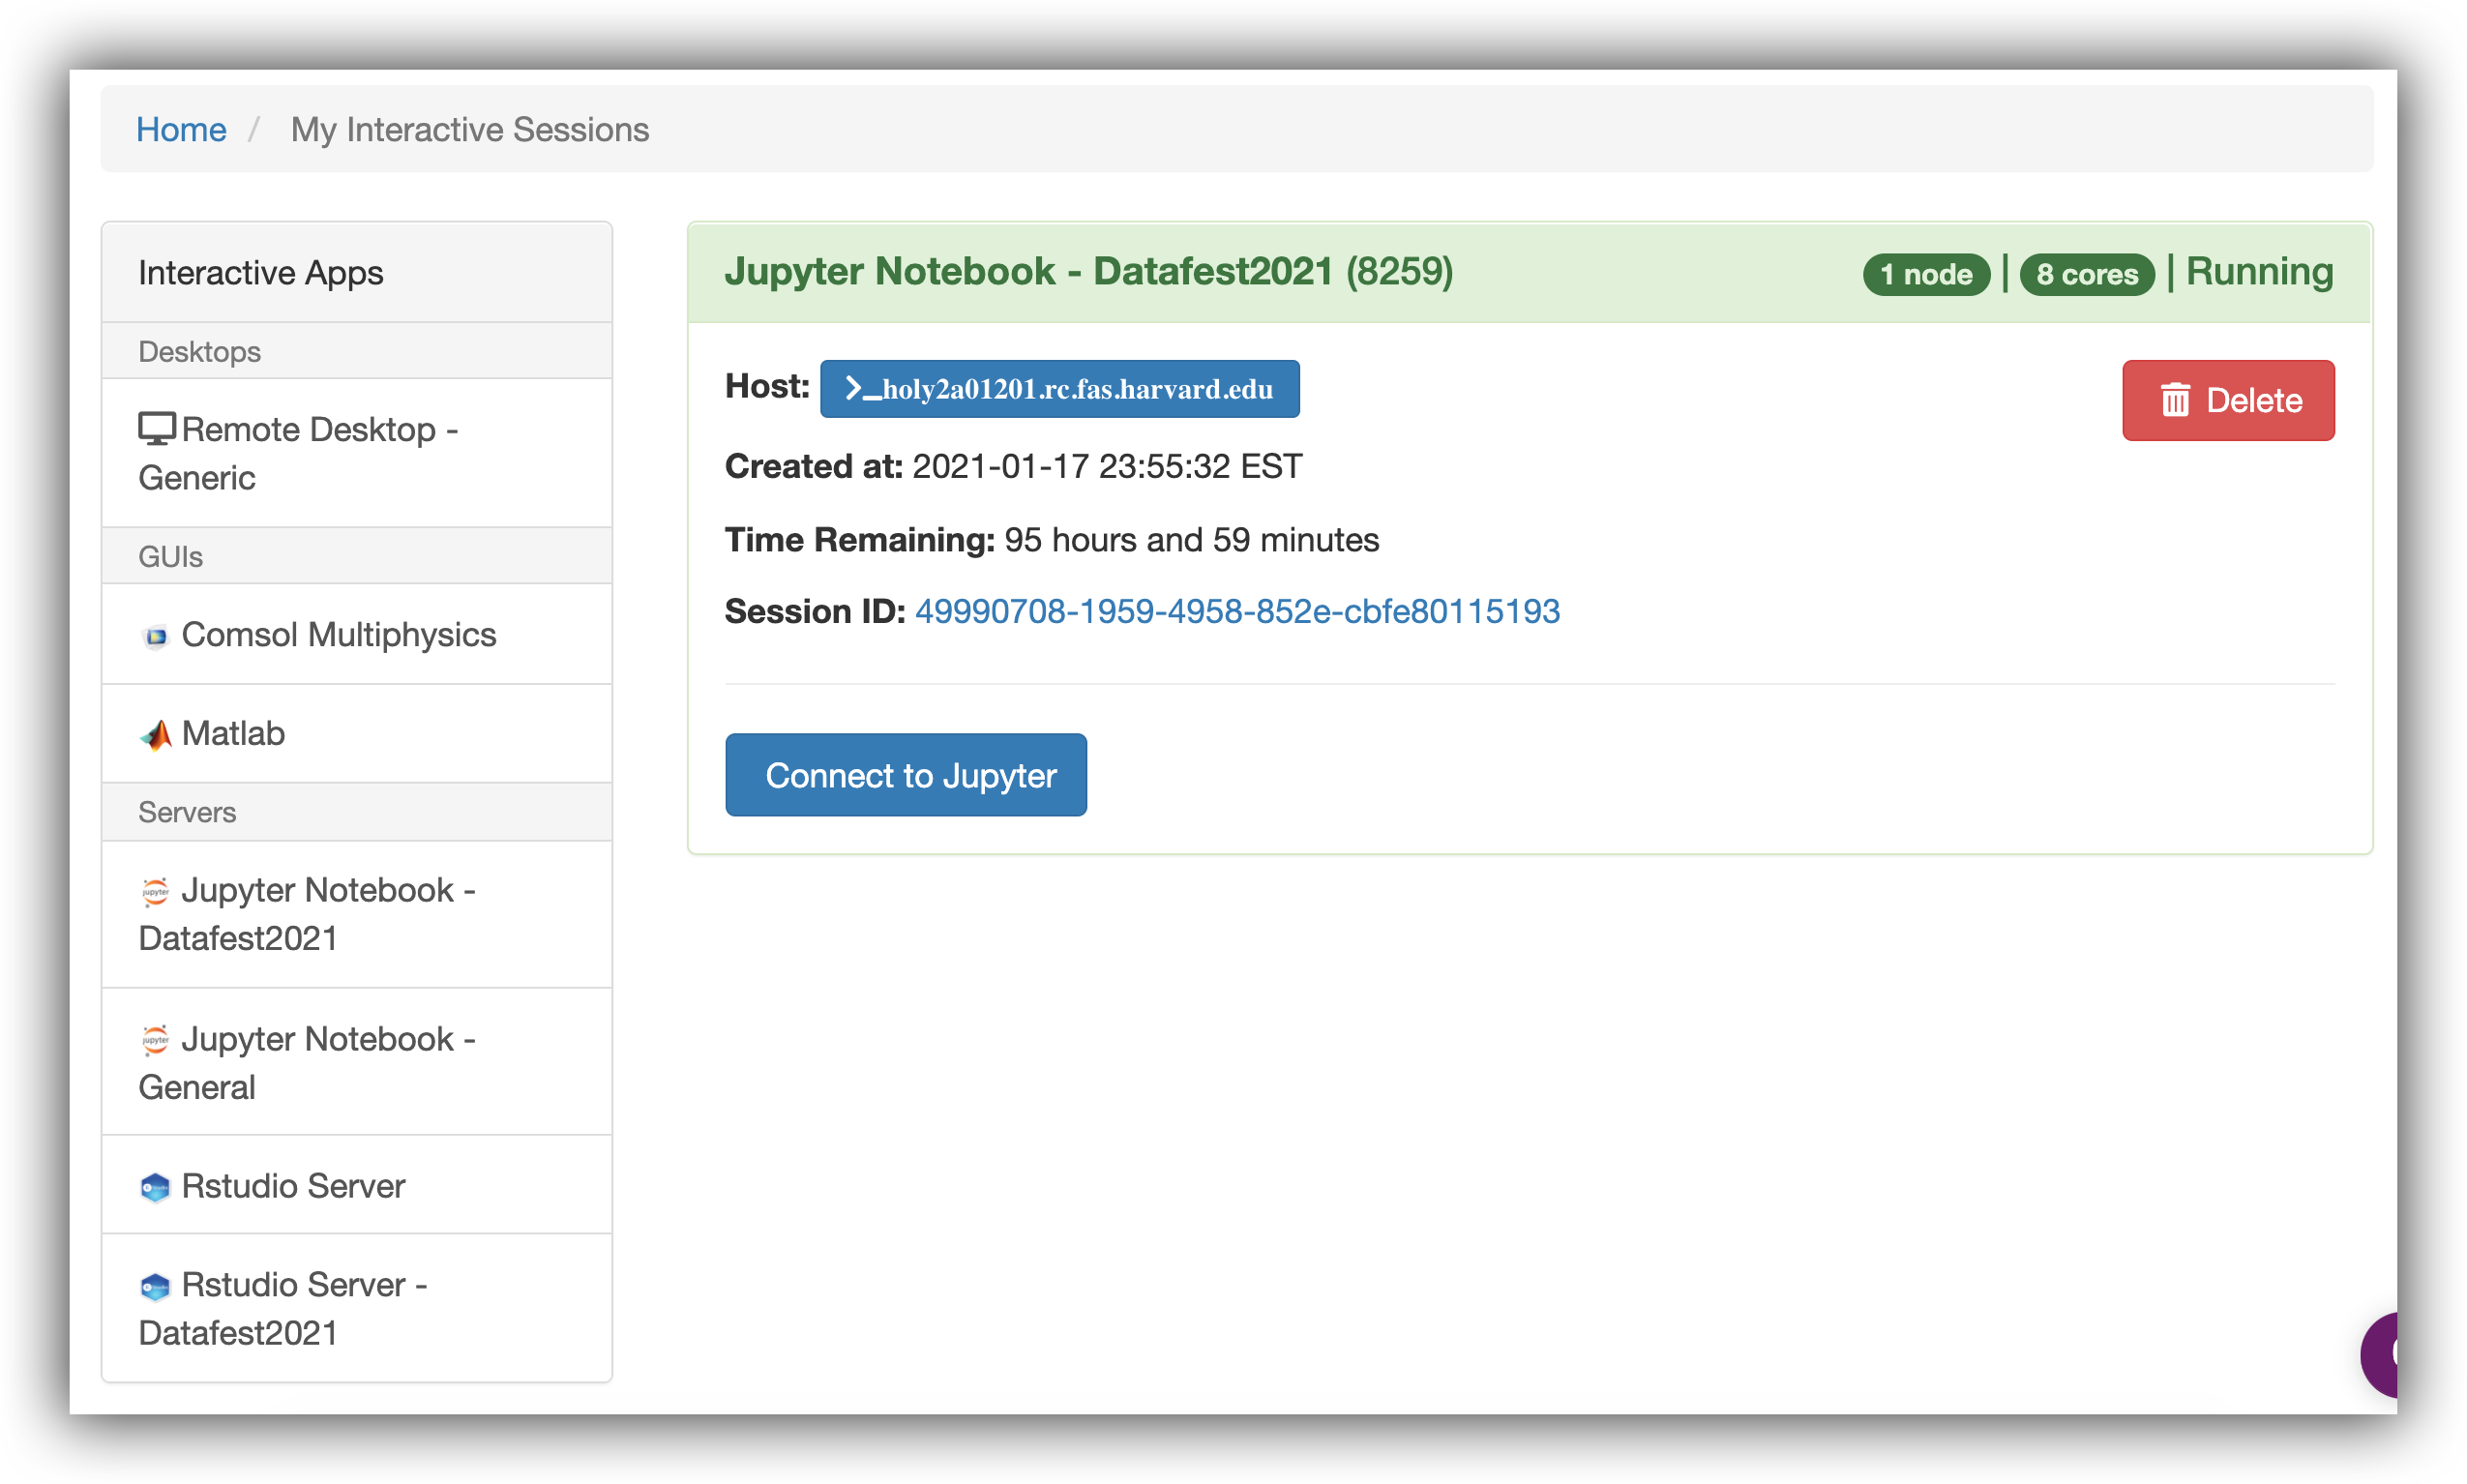
\includegraphics{images/5_connect_jupyter.png}

\begin{enumerate}
\def\labelenumi{\arabic{enumi}.}
\setcounter{enumi}{4}
\tightlist
\item
  You should now have access to Jupyter. You can either create a new notebook from the \texttt{New} dropdown on the far right (select the \texttt{datafest\_2021} kernel) or you can navigate to an existing file (after opening the file, select the \texttt{datafest\_2021} kernel from the Kernal menu).
\end{enumerate}

\hypertarget{copy-instructors-codedata-to-your-home-directory}{%
\chapter{Copy instructor's code/data to your home directory}\label{copy-instructors-codedata-to-your-home-directory}}

If your instructor has uploaded code and/or data to the shared drive (this is the \texttt{shared\_data} directory within your \texttt{Home} directory) then the first thing you should do before using these files is to copy them to your \texttt{Home} directory. These copies will serve as your own personal version of the files, which you can modify as you wish.

There are several different ways you can copy files from the \texttt{shared\_data} directory to your \texttt{Home} directory, depending on whether you'd prefer to use the command line or a GUI. Here are the options:

\hypertarget{rstudio-1}{%
\section{RStudio}\label{rstudio-1}}

\hypertarget{using-terminal}{%
\subsection{Using Terminal}\label{using-terminal}}

\begin{enumerate}
\def\labelenumi{\arabic{enumi}.}
\tightlist
\item
  Click on the \texttt{Terminal} tab on the top left panel, next to \texttt{Console}.
\item
  Copy the file(s) or directories you want from the ``shared\_data'' directory to your home directory: \texttt{cp\ -r\ shared\_data/\textless{}directory-you-want\textgreater{}/\ .}
\end{enumerate}

\hypertarget{using-shell-commands-in-the-r-console}{%
\subsection{Using shell commands in the R console}\label{using-shell-commands-in-the-r-console}}

\begin{enumerate}
\def\labelenumi{\arabic{enumi}.}
\tightlist
\item
  Copy the file(s) or directories you want from the \texttt{shared\_data} directory to your home directory by running the following command in the console: \texttt{system("cp\ -r\ \textasciitilde{}/shared\_data/\textless{}directory-you-want\textgreater{}/\ .")}
\end{enumerate}

\hypertarget{using-the-file-menu}{%
\subsection{Using the File menu}\label{using-the-file-menu}}

\begin{enumerate}
\def\labelenumi{\arabic{enumi}.}
\tightlist
\item
  In the \texttt{Files} menu in the bottom right panel, navigate to the \texttt{shared\_data} directory.
\item
  Navigate to the directory with materials for the current session.
\item
  Put a check next to the file you want to copy to your home folder. You can only copy one file at a time and no directories.
\item
  Click on the \texttt{More} dropdown menu (with gears icon) and select \texttt{Copy\ To}.
\item
  Near the top of the resulting pop-up window, click on the \texttt{Home} directory icon.
\item
  Click the \texttt{Save} button on the bottom right. There will now be a copy of the file in your home directory, which you can open and work with.
\end{enumerate}

\hypertarget{jupyter-1}{%
\section{Jupyter}\label{jupyter-1}}

\hypertarget{using-terminal-1}{%
\subsection{Using Terminal}\label{using-terminal-1}}

\begin{enumerate}
\def\labelenumi{\arabic{enumi}.}
\tightlist
\item
  Click on the \texttt{New} dropdown on the right side of the page.
\item
  Select \texttt{Terminal} from the dropdown menu.
\item
  In the new browser tab, copy the file(s) or directories you want from the \texttt{shared\_data} directory to your home directory: \texttt{cp\ -r\ shared\_data/\textless{}directory-you-want\textgreater{}/\ .}
\item
  Close the browser tab containing the Terminal (don't click \texttt{logout}!). Go back to the previous browser tab to access Jupyter again.
\end{enumerate}

\hypertarget{using-shell-commands-in-cells}{%
\subsection{Using shell commands in cells}\label{using-shell-commands-in-cells}}

\begin{enumerate}
\def\labelenumi{\arabic{enumi}.}
\tightlist
\item
  Open a Jupyter Notebook or create a new cell.
\item
  Copy the file(s) of interest to your home directory: \texttt{!cp\ -r\ \textasciitilde{}/shared\_data/\textless{}directory-you-want\textgreater{}/\ .}
\end{enumerate}

\hypertarget{using-the-file-menu-1}{%
\subsection{Using the File menu}\label{using-the-file-menu-1}}

\begin{enumerate}
\def\labelenumi{\arabic{enumi}.}
\tightlist
\item
  Navigate to the file of interest within the \texttt{shared\_data} directory.
\item
  Click \texttt{Duplicate} from the top menu.
\item
  Select the radio button next to the duplicated file.
\item
  Click \texttt{Move} from the top menu.
\item
  Delete ALL of the file path in the pop-up window and click the blue \texttt{Move} button
\end{enumerate}

\hypertarget{download-codedata-to-your-personal-computer}{%
\chapter{Download code/data to your personal computer}\label{download-codedata-to-your-personal-computer}}

At the end of your project, you will probably want to download your script files and data files from the FAS OnDemand environment to your local machine. This is easy to do from within RStudio / Jupyter:

\hypertarget{rstudio-2}{%
\section{RStudio}\label{rstudio-2}}

\begin{enumerate}
\def\labelenumi{\arabic{enumi}.}
\tightlist
\item
  Select the file of interest using the radio button within the file browser (bottom right panel).
\item
  Click on the \texttt{More} dropdown menu (with gears icon) and select \texttt{Export}.
\item
  In the pop-up window, click \texttt{Download}.
\end{enumerate}

\hypertarget{jupyter-2}{%
\section{Jupyter}\label{jupyter-2}}

\begin{enumerate}
\def\labelenumi{\arabic{enumi}.}
\tightlist
\item
  Select the file of interest using the radio button within the file browser.
\item
  Click the \texttt{Download} button on the top menu.
\end{enumerate}

\hypertarget{upload-codedata-to-your-home-directory}{%
\chapter{Upload code/data to your home directory}\label{upload-codedata-to-your-home-directory}}

If you have files on your personal computer that you'd like to use within the FAS OnDemand computing environment, you can upload them by following these steps (the steps are the same regardless of whether you intend to use RStudio or Jupyter):

\begin{enumerate}
\def\labelenumi{\arabic{enumi}.}
\tightlist
\item
  Click \texttt{FAS\ OnDemand} in the left-side navigation panel within Canvas.
\item
  On the Dashboard launcher page, go to the \texttt{Files} dropdown menu at top-left and click on \texttt{Home\ Directory}.
\item
  Within the File Explorer page, click on the \texttt{Go\ To} button in the top most menu and navigate to: \texttt{/n/academic\_homes/g\_87116/SHARE/shared\_data/} Note: this location for \texttt{shared\_data} has been symlinked to your \texttt{Home} directory, so you will also see, and be able to access files from, \texttt{shared\_data} within \texttt{Home}.
\item
  Within the \texttt{shared\_data} directory, you can upload whatever code/data files you and your participants will need by clicking on the \texttt{Upload} button at the very top of the page and then choosing a file from your local machine. It probably makes sense to organize your files by first creating a directory with a short-named version of your demo session (see the \texttt{New\ Dir} button in the very top most menu). Make sure not to leave spaces in the directory name - use underscores (e.g., \texttt{APIs\_to\_acquire\_data}). Then upload your files into this directory.
\end{enumerate}

\end{document}
